%Introducci�n al cap�tulo

%--------------------------------------------------
\section{Objetivos}

% - - - - - - - - - - - - - - - - - - - - - - - - -
\subsection{Objetivo general}

Crear un sistema en el que puedan solucionar las problematicas principales en una cl\'inica m\'edica, tanto en la cl\'inica como en el sitio web.


% - - - - - - - - - - - - - - - - - - - - - - - - -
\subsection{Objetivos espec�ficos}

\begin{itemize}
	\item Llevar a cabo el proceso de citas por internet, donde el paciente podra seleccionar el tipo de consulta (Especialidad o General) y fecha en la que se solicitar\'a dicha cita.
	\item Manejar una base de datos para contener los expedientes m\'edicos (Informaci\'on General) de los pacientes que tengan consulta.
	\item Tener control e informar sobre el manejo interno en farmacia (Inventario y Surtido).
	\item Informar\'a al cliente si la cita puede realizarse con base a la disponibilidad de consultorios. En caso de que esten agotada en una determinada fecha, el paciente podra reprogramar la cita.
\end{itemize}


%--------------------------------------------------
\section{Modelo de despliegue}


% - - - - - - - - - - - - - - - - - - - - - - - - -
\subsection{Requerimientos no funcionales}

\begin{table}[h]
\hspace{-.50cm}
\begin{tabular}{|l|l|l|}
\hline
	\multicolumn{1}{|c|}{\textbf{ID}} & \multicolumn{1}{c|}{\textbf{Nombre}} & \multicolumn{1}{c|}{\textbf{Descripci\'on}} \\ \hline
	RNF1 & Forma de almacenamiento & \begin{tabular}[c]{@{}l@{}}La informaci\'on requerida se guardar\'a en una base de datos de MySQL
																														 \end{tabular} \\ \hline
	RNF2	& Cupo de horario & \begin{tabular}[c]{@{}l@{}}Mediante consultas de SQL, la plataforma web determinar\'a si es posible realizar\\una cita en el horario seleccionado
																											 \end{tabular} \\ \hline
	RNF3 & Tecnolog\'ias web & \begin{tabular}[c]{@{}l@{}}Para la plataforma web se usar\'an las tecnolog\'ias HTML, CSS y PHP
																													 \end{tabular} \\ \hline
	RNF4 & \begin{tabular}[c]{@{}l@{}}Selecci\'on de horario \end{tabular} & 
	\begin{tabular}[c]{@{}l@{}}El sistema le mostrar\'a al usuario los horarios disponibles \\ en intervalos de media hora. \end{tabular} \\ \hline
																															
\end{tabular}
\end{table}



% - - - - - - - - - - - - - - - - - - - - - - - - -
\subsection{Modelo de despliegue del sistema}

Diagrama de despliegue presentando los sistemas (comunicaciones, sistemas externos y software de base) con los que interact�a el sistema y su explicaci�n. vea los siguientes cuatro ejemplos.

	\begin{figure}[htbp!]
		\centering
			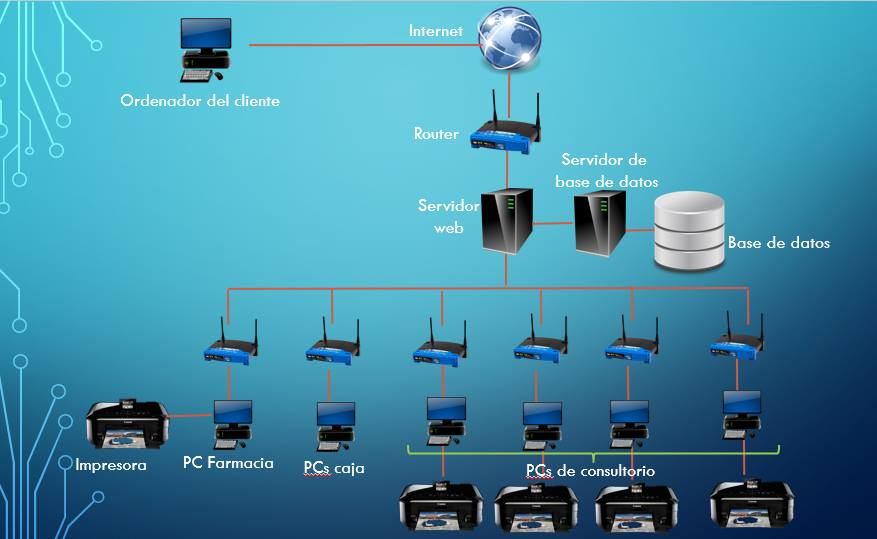
\includegraphics[width=0.8\textwidth]{images/df}
		\caption{Diagrama de arquitectura.}
	\end{figure}

	%\begin{figure}[htbp!]
	%	\centering
	%		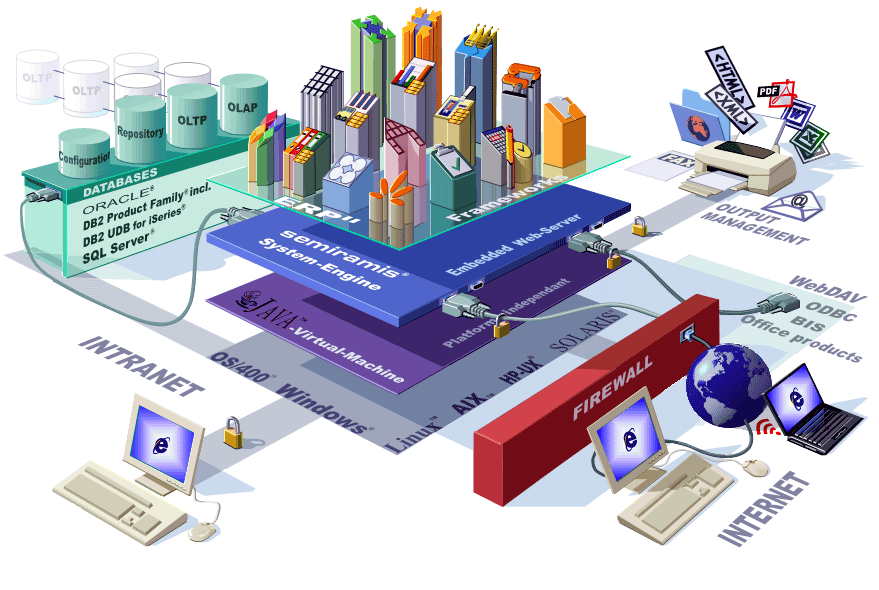
\includegraphics[width=0.8\textwidth]{images/arquitectura2}
	%	\caption{Diagrama de arquitectura.}
	%\end{figure}

	%\begin{figure}[htbp!]
	%	\centering
	%		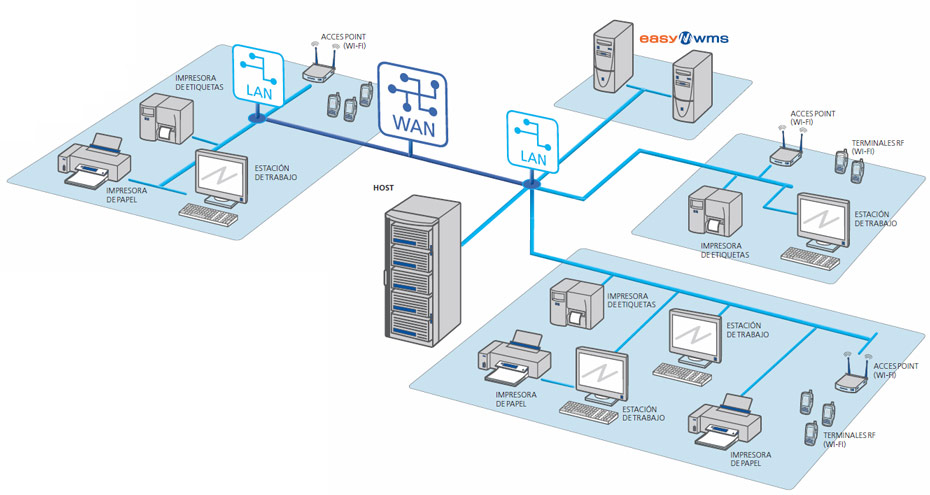
\includegraphics[width=0.8\textwidth]{images/arquitectura3}
	%	\caption{Diagrama de arquitectura.}
	%\end{figure}

	%\begin{figure}[htbp!]
	%	\centering
	%		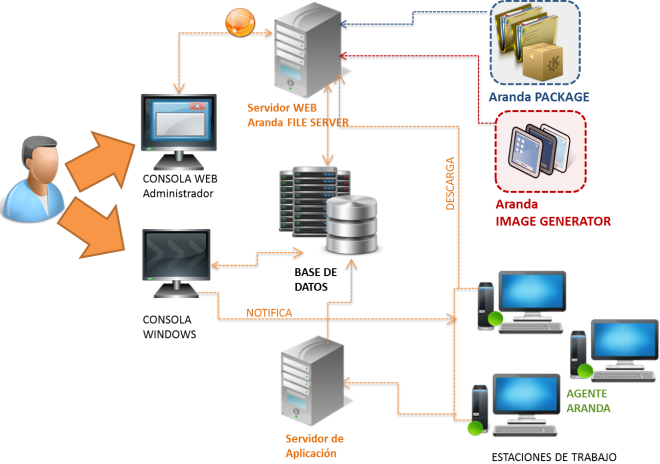
\includegraphics[width=0.8\textwidth]{images/arquitectura4}
	%	\caption{Diagrama de arquitectura.}
	%\end{figure}


% - - - - - - - - - - - - - - - - - - - - - - - - -
\subsection{Especificaci�n de Plataforma}

%Especificar, hardware, software y servicios requeridos para el sistema.

\begin{description}
    \item[Ordenador cliente]
\end{description}
    
\begin{description}
    \item[Servidor]
\end{description}

\begin{description}
    \item[Servidor]
\end{description}

\begin{description}
    \item[Base de Datos]
\end{description}

\begin{description}
    \item[PC Farmacia]
\end{description}

\begin{description}
    \item[PC Caja]
\end{description}

\begin{description}
    \item[PC Consultorio]
\end{description}

\begin{description}
    \item[Impresoras]
\end{description}